\documentclass{book}
\usepackage[a4paper,top=2.5cm,bottom=2.5cm,left=2.5cm,right=2.5cm]{geometry}
\usepackage{makeidx}
\usepackage{natbib}
\usepackage{graphicx}
\usepackage{multicol}
\usepackage{float}
\usepackage{listings}
\usepackage{color}
\usepackage{ifthen}
\usepackage[table]{xcolor}
\usepackage{textcomp}
\usepackage{alltt}
\usepackage{ifpdf}
\ifpdf
\usepackage[pdftex,
            pagebackref=true,
            colorlinks=true,
            linkcolor=blue,
            unicode
           ]{hyperref}
\else
\usepackage[ps2pdf,
            pagebackref=true,
            colorlinks=true,
            linkcolor=blue,
            unicode
           ]{hyperref}
\usepackage{pspicture}
\fi
\usepackage[utf8]{inputenc}
\usepackage[french]{babel}

\usepackage{mathptmx}
\usepackage[scaled=.90]{helvet}
\usepackage{courier}
\usepackage{sectsty}
\usepackage{amssymb}
\usepackage[titles]{tocloft}
\usepackage{doxygen}
\lstset{language=C++,inputencoding=utf8,basicstyle=\footnotesize,breaklines=true,breakatwhitespace=true,tabsize=8,numbers=left }
\makeindex
\setcounter{tocdepth}{3}
\renewcommand{\footrulewidth}{0.4pt}
\renewcommand{\familydefault}{\sfdefault}
\hfuzz=15pt
\setlength{\emergencystretch}{15pt}
\hbadness=750
\tolerance=750
\begin{document}
\hypersetup{pageanchor=false,citecolor=blue}
\begin{titlepage}
\vspace*{7cm}
\begin{center}
{\Large Lesson01 }\\
\vspace*{1cm}
{\large Généré par Doxygen 1.8.3.1}\\
\vspace*{0.5cm}
{\small Dimanche Mai 12 2013 16:09:57}\\
\end{center}
\end{titlepage}
\clearemptydoublepage
\pagenumbering{roman}
\tableofcontents
\clearemptydoublepage
\pagenumbering{arabic}
\hypersetup{pageanchor=true,citecolor=blue}
\chapter{Index des fichiers}
\section{Liste des fichiers}
Liste de tous les fichiers documentés avec une brève description \-:\begin{DoxyCompactList}
\item\contentsline{section}{\hyperlink{_lesson01_8c}{Lesson01.\-c} \\*Ouvre une simple fen�tre Windows et dessine un triangle muticolore en rotation avec Open\-G\-L }{\pageref{_lesson01_8c}}{}
\end{DoxyCompactList}

\chapter{Documentation des fichiers}
\doxysection{Lesson01.\+c File Reference}
\label{_lesson01_8c}\index{Lesson01.c@{Lesson01.c}}


Ouvre une simple fen�tre Windows et dessine un triangle muticolore en rotation avec Open\+GL.  


{\ttfamily \#include $<$windows.\+h$>$}\newline
{\ttfamily \#include $<$gl/gl.\+h$>$}\newline
{\ttfamily \#include \char`\"{}resource.\+h\char`\"{}}\newline
Include dependency graph for Lesson01.\+c\+:
\nopagebreak
\begin{figure}[H]
\begin{center}
\leavevmode
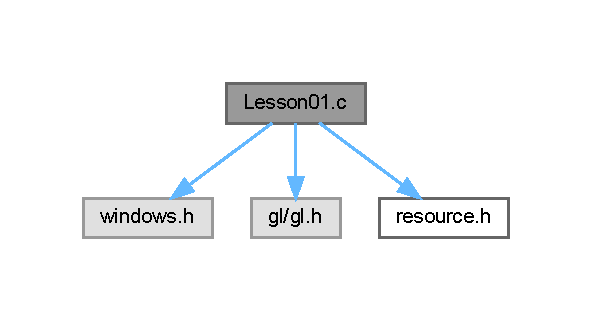
\includegraphics[width=284pt]{_lesson01_8c__incl}
\end{center}
\end{figure}
\doxysubsection*{Macros}
\begin{DoxyCompactItemize}
\item 
\#define \textbf{ WIN32\+\_\+\+LEAN\+\_\+\+AND\+\_\+\+MEAN}
\end{DoxyCompactItemize}
\doxysubsection*{Functions}
\begin{DoxyCompactItemize}
\item 
LRESULT CALLBACK \textbf{ Window\+Proc} (HWND hwnd, UINT u\+Msg, WPARAM w\+Param, LPARAM l\+Param)
\begin{DoxyCompactList}\small\item\em Fonction CALLBACK de traitement des messages Windows. \end{DoxyCompactList}\item 
void \textbf{ Enable\+Open\+GL} (HWND hwnd, HDC $\ast$h\+DC, HGLRC $\ast$h\+RC)
\begin{DoxyCompactList}\small\item\em Fonction Enable\+Open\+GL permettant la configuration d\textquotesingle{}Open\+GL pour la fen�tre principale. \end{DoxyCompactList}\item 
void \textbf{ Disable\+Open\+GL} (HWND hwnd, HDC h\+DC, HGLRC h\+RC)
\begin{DoxyCompactList}\small\item\em Fonction Disable\+Open\+GL permettant la d�-\/configuration d\textquotesingle{}Open\+GL pour la fen�tre principale. \end{DoxyCompactList}\item 
int WINAPI \textbf{ Win\+Main} (HINSTANCE h\+Instance, HINSTANCE h\+Prev\+Instance, LPSTR lp\+Cmd\+Line, int n\+Cmd\+Show)
\begin{DoxyCompactList}\small\item\em Fonction Win\+Main obligatoire pour les programmes utilisant l\textquotesingle{}UI Windows. \end{DoxyCompactList}\end{DoxyCompactItemize}


\doxysubsection{Detailed Description}
Ouvre une simple fen�tre Windows et dessine un triangle muticolore en rotation avec Open\+GL. 

Comments manageable by Doxygen

Modified smoothly by Thierry DECHAIZE

Paradigm \+: obtain one source (only one !) compatible for multiple free C Compilers and provide for all users an development environment on Windows (64 bits compatible), the great Code\+::\+Blocks manager (version 20.\+03), and don\textquotesingle{}t use glaux.\+lib or glaux.\+dll.

a) Mingw 32 bits, version officielle gcc 9.\+2.\+0 (very old !) \+: downloadable on {\texttt{ http\+://sourceforge.\+net/projects/mingw/}} (official) b) Mingw 64 bits included in new IDE Red Panda Dev-\/\+Cpp, version gcc 12.\+2.\+0 \+: donwloadable on {\texttt{ https\+://sourceforge.\+net/projects/redpanda-\/cpp/files/}} c) Mingw 64 bits included in package Code\+::\+Blocks (version 20.\+03 with mingw), version gcc 11.\+2.\+0 \+: downloadable on {\texttt{ http\+://sourceforge.\+net/projects/codeblocks/files/\+Binaries/20.\+03/\+Windows/}} d) Mingw 32 and 64 bits packag�s, version gcc 11.\+2.\+0 \+: downloadable on {\texttt{ https\+://winlibs.\+com/}} (and CLANG included in, 32 and 64 bits), two kits \+:
\begin{DoxyItemize}
\item winlibs-\/i686-\/posix-\/dwarf-\/gcc-\/12.\+2.\+0-\/llvm-\/15.\+0.\+7-\/mingw-\/w64ucrt-\/10.\+0.\+0-\/r4.\+7z (32 bits)
\item winlibs-\/x86\+\_\+64-\/posix-\/seh-\/gcc-\/12.\+2.\+0-\/llvm-\/15.\+0.\+7-\/mingw-\/w64ucrt-\/10.\+0.\+0-\/r4.\+7z (64 bits) e) Cygwin64, 32 et 64 bits, version gcc 11.\+3.\+0 \+: downloadable on {\texttt{ http\+://www.\+cygwin.\+com/install.\+html}} (tool for install \+: setup-\/x86\+\_\+64.\+exe) f) TDM GCC, 32 et 64 bits, version 10.\+3.\+0 \+: downloadable on {\texttt{ http\+://sourceforge.\+net/projects/\+TDM-\/\+GCC}} g) MSYS2 environnement MINGW32 and MINGW64, 32 et 64 bits, version de 2022 (msys2-\/x86\+\_\+64-\/20230127.\+exe), version gcc 12.\+2.\+0 \+: downloadable on {\texttt{ https\+://repo.\+msys2.\+org/distrib/x86\+\_\+64/msys2-\/x86\+\_\+64-\/20230127.\+exe}} h) Visual Studio 2022, 32 et 64 bits, community edition for free \+: downloadable on {\texttt{ https\+://visualstudio.\+microsoft.\+com/fr/thank-\/you-\/downloading-\/visual-\/studio/?sku=\+Community\&rel=17}} i) Borland C/\+C++ 32 bits, version 5.\+5 \+: downloadable on {\texttt{ https\+://developerinsider.\+co/download-\/and-\/install-\/borland-\/c-\/compiler-\/on-\/windows-\/10/}} j) Digital Mars Compiler C 32 bits version 8.\+57 \+: downloadable on {\texttt{ http\+://www.\+digitalmars.\+com}} (the more old compiler, the more bugged, dead branch !) k) Open\+Watcom 32 et 64 bits, version 2.\+0 \+: downloadable on {\texttt{ http\+://openwatcom.\+mirror.\+fr/}} l) Lcc and Lcc64, 32 et 64 bits\+: downloadable {\texttt{ http\+://www.\+cs.\+virginia.\+edu/$\sim$lcc-\/win32/}} m) PELLES C, 32 et 64 bits, version 11.\+0 \+: downloadable on {\texttt{ http\+://www.\+smorgasbordet.\+com/pellesc/}} o) CLANG, adoss� aux environnements MINGW64 et MINGW32, version 15.\+0.\+7 (version gcc 12.\+0.\+0) \+: downloadable on {\texttt{ https\+://winlibs.\+com/}} p) CLANG, adoss� aux environnements Visual Studio 2022 (+ kits Microsoft), version 15.\+0.\+7 \+: downloadable on {\texttt{ https\+://releases.\+llvm.\+org/download.\+html}} q) CLANG de la version MSYS2, adoss� aux environnements MINGW64 et MINGW32, version 15.\+0.\+7 (version gcc 12.\+2.\+0) \+: downloadable on {\texttt{ https\+://repo.\+msys2.\+org/distrib/x86\+\_\+64/msys2-\/x86\+\_\+64-\/20220118.\+exe}} r) CLANG de la version CYGWIN, adoss� aux environnements MINGW64 et MINGW32, version 8.\+0.\+0 (version gcc 11.\+3.\+0) \+: downloadable {\texttt{ http\+://www.\+cygwin.\+com/install.\+html}} (tool for install \+: setup-\/x86\+\_\+64.\+exe)
\end{DoxyItemize}

TDE -\/$>$ Add resource file end resource header for restitute version + icon Open\+GL.\+ico for fun because versionning is important, same for freeware \+:-\/) !

Date \+: 2023/02/03

\begin{DoxyAuthor}{Author}
Jeff Molofee ( Ne\+He ) originely, adapted by Thierry Dechaize 
\end{DoxyAuthor}
\begin{DoxyVersion}{Version}
2.\+0.\+1.\+0 
\end{DoxyVersion}
\begin{DoxyDate}{Date}
3 f�vrier 2023
\end{DoxyDate}
Ce programme ne g�re que deux �v�nements \+: le clic sur le bouton \char`\"{}\+Ferm�\char`\"{} de la fen�tre ou la sortie par la touche ESC. 

\doxysubsection{Macro Definition Documentation}
\mbox{\label{_lesson01_8c_ac7bef5d85e3dcd73eef56ad39ffc84a9}} 
\index{Lesson01.c@{Lesson01.c}!WIN32\_LEAN\_AND\_MEAN@{WIN32\_LEAN\_AND\_MEAN}}
\index{WIN32\_LEAN\_AND\_MEAN@{WIN32\_LEAN\_AND\_MEAN}!Lesson01.c@{Lesson01.c}}
\doxysubsubsection{WIN32\_LEAN\_AND\_MEAN}
{\footnotesize\ttfamily \#define WIN32\+\_\+\+LEAN\+\_\+\+AND\+\_\+\+MEAN}



\doxysubsection{Function Documentation}
\mbox{\label{_lesson01_8c_a90bd4ce009c06870ec5a57a16b8d7b3a}} 
\index{Lesson01.c@{Lesson01.c}!DisableOpenGL@{DisableOpenGL}}
\index{DisableOpenGL@{DisableOpenGL}!Lesson01.c@{Lesson01.c}}
\doxysubsubsection{DisableOpenGL()}
{\footnotesize\ttfamily void Disable\+Open\+GL (\begin{DoxyParamCaption}\item[{HWND}]{hwnd,  }\item[{HDC}]{h\+DC,  }\item[{HGLRC}]{h\+RC }\end{DoxyParamCaption})}



Fonction Disable\+Open\+GL permettant la d�-\/configuration d\textquotesingle{}Open\+GL pour la fen�tre principale. 

Comments manageable by Doxygen

On lib�re les diff�rents contextes \+: Device Context et Resource Context. 
\begin{DoxyParams}{Parameters}
{\em hwnd} & L\textquotesingle{}header de la fen�tre principale. \\
\hline
{\em h\+DC} & L\textquotesingle{}header du Device Context. \\
\hline
{\em h\+RC} & L\textquotesingle{}header du Resource Context sous Open\+GL. \\
\hline
\end{DoxyParams}
Here is the caller graph for this function\+:
\nopagebreak
\begin{figure}[H]
\begin{center}
\leavevmode
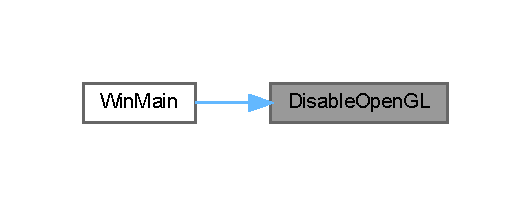
\includegraphics[width=255pt]{_lesson01_8c_a90bd4ce009c06870ec5a57a16b8d7b3a_icgraph}
\end{center}
\end{figure}
\mbox{\label{_lesson01_8c_a3f1d8020cc3dcf306710f0e74385d3b4}} 
\index{Lesson01.c@{Lesson01.c}!EnableOpenGL@{EnableOpenGL}}
\index{EnableOpenGL@{EnableOpenGL}!Lesson01.c@{Lesson01.c}}
\doxysubsubsection{EnableOpenGL()}
{\footnotesize\ttfamily void Enable\+Open\+GL (\begin{DoxyParamCaption}\item[{HWND}]{hwnd,  }\item[{HDC $\ast$}]{h\+DC,  }\item[{HGLRC $\ast$}]{h\+RC }\end{DoxyParamCaption})}



Fonction Enable\+Open\+GL permettant la configuration d\textquotesingle{}Open\+GL pour la fen�tre principale. 

Comments manageable by Doxygen

Ce qui est important est le descripteur du format du pixel utilis�. 
\begin{DoxyParams}{Parameters}
{\em hwnd} & L\textquotesingle{}header de la fen�tre principale. \\
\hline
{\em h\+DC} & L\textquotesingle{}header du Device Context. \\
\hline
{\em h\+RC} & L\textquotesingle{}header du Resource Context sous Open\+GL. \\
\hline
\end{DoxyParams}
Here is the caller graph for this function\+:
\nopagebreak
\begin{figure}[H]
\begin{center}
\leavevmode
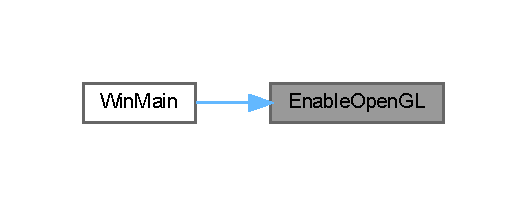
\includegraphics[width=253pt]{_lesson01_8c_a3f1d8020cc3dcf306710f0e74385d3b4_icgraph}
\end{center}
\end{figure}
\mbox{\label{_lesson01_8c_af7de05620634745d22ea79adeef2514f}} 
\index{Lesson01.c@{Lesson01.c}!WindowProc@{WindowProc}}
\index{WindowProc@{WindowProc}!Lesson01.c@{Lesson01.c}}
\doxysubsubsection{WindowProc()}
{\footnotesize\ttfamily LRESULT CALLBACK Window\+Proc (\begin{DoxyParamCaption}\item[{HWND}]{hwnd,  }\item[{UINT}]{u\+Msg,  }\item[{WPARAM}]{w\+Param,  }\item[{LPARAM}]{l\+Param }\end{DoxyParamCaption})}



Fonction CALLBACK de traitement des messages Windows. 

Comments manageable by Doxygen

Traitement de la boucle infinie des messages Windows 
\begin{DoxyParams}{Parameters}
{\em hwnd} & L\textquotesingle{}header de la fen�tre principale. \\
\hline
{\em u\+Msg} & Un entier non sign�. \\
\hline
{\em w\+Param} & Les param�tres en entr�e. \\
\hline
{\em l\+Param} & Autres param�tres en entr�e. \\
\hline
\end{DoxyParams}
\begin{DoxyReturn}{Returns}
LRESULT Un LRESULT donnant le status du traitement du message. 
\end{DoxyReturn}
Here is the caller graph for this function\+:
\nopagebreak
\begin{figure}[H]
\begin{center}
\leavevmode
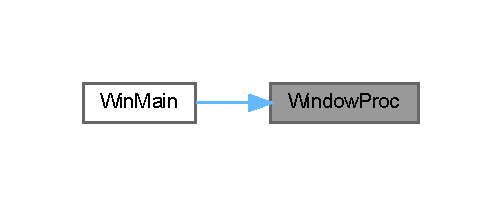
\includegraphics[width=241pt]{_lesson01_8c_af7de05620634745d22ea79adeef2514f_icgraph}
\end{center}
\end{figure}
\mbox{\label{_lesson01_8c_a661c2abc03926acfaeb93b4ae7db4943}} 
\index{Lesson01.c@{Lesson01.c}!WinMain@{WinMain}}
\index{WinMain@{WinMain}!Lesson01.c@{Lesson01.c}}
\doxysubsubsection{WinMain()}
{\footnotesize\ttfamily int WINAPI Win\+Main (\begin{DoxyParamCaption}\item[{HINSTANCE}]{h\+Instance,  }\item[{HINSTANCE}]{h\+Prev\+Instance,  }\item[{LPSTR}]{lp\+Cmd\+Line,  }\item[{int}]{n\+Cmd\+Show }\end{DoxyParamCaption})}



Fonction Win\+Main obligatoire pour les programmes utilisant l\textquotesingle{}UI Windows. 

Comments manageable by Doxygen

Creation de la fenetre principale 
\begin{DoxyParams}{Parameters}
{\em h\+Instance} & L\textquotesingle{}header de l\textquotesingle{}instance de la fen�tre principale. \\
\hline
{\em h\+Prev\+Instance} & L\textquotesingle{}header de l\textquotesingle{}instance de la fen�tre pr�c�dente (si besoin). \\
\hline
{\em lp\+Cmd\+Line} & Un pointeur sur la ligne de cammande. \\
\hline
{\em n\+Cmd\+Show} & Un indicateur. \\
\hline
\end{DoxyParams}
\begin{DoxyReturn}{Returns}
int Le status du lancement et de la creation de la fen�tre (ok ou non). 
\end{DoxyReturn}
Here is the call graph for this function\+:
\nopagebreak
\begin{figure}[H]
\begin{center}
\leavevmode
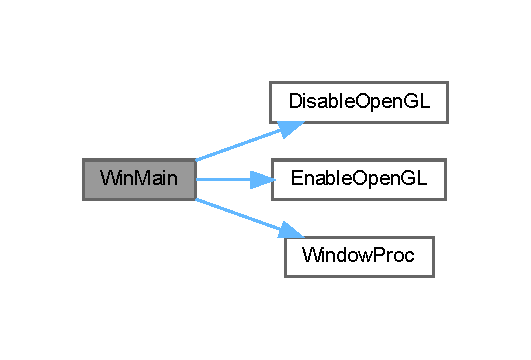
\includegraphics[width=255pt]{_lesson01_8c_a661c2abc03926acfaeb93b4ae7db4943_cgraph}
\end{center}
\end{figure}

\addcontentsline{toc}{part}{Index}
\printindex
\end{document}
